\chapter[Data Augmentation with Generative Adversarial
Networks]{Data Augmentation with \\ Generative Adversarial
Networks}
% \begin{markdown}
% ---

% - We are coming from the simulation chapter, so:
% - Problem description: 
%  - We would like to produce larger amounts of simulation data, e.g. for a mock
%    dataset in preparation for data-taking
%  - But we have limited capability to produce MC data with simulation. The main
%    bottleneck is in the pion-production section's hadronic interactions. Is
%    there a faster way?
%   - The topic of this chapter is to consider the application of
%     machine-learning methods in the fabrication of fake Monte Carlo data.


% - Creation of dataset from Monte Carlo simulation
%   - Hit pattern characterisation
%   - Reconstructible vs noise-like classification
% - GAN theory [Goodfellow, WGAN, WGAN-GP]
%  - Pre-processing
% - GAN design, basic architecture, softmax for classes [WGAN-GP]
% - GAN extensions, embedding? analogy with text?

% ---
% \end{markdown}

% Need to wrap the start of this chapter into a compelling narrative:
% 1. MC allows us to see possible patterns in detector sys e.g., in CDC,
%    high-mom tracks produce structured hits whereas low-mom make small
%    localised hit clusters --> Draw figures
% 2. For an exercise such as a mock-data challenge (explain term), traditional
%    MC is not efficient enough to produce the dataset.
%  + Think about: why do we want mock data? Why is the standard sensitivity
%    estimation process not sufficient?
%    - Perhaps the extrapolation factor. Considering efficiencies on a limited
%       sample cannot effectively be representative of the real situation.
%    - The sheer sample size makes the exercise worth it? Test limits of the
%       data processing chain and increase preparedness for real situation.
% 3. Now consider the problem of producing artificial / fake / imitation /
%    fictitious / fabricated data.
%  + Consider alternatives
%  + Introduce GAN for detector-level data fabrication.


% v -- This intro is plain useless I think. 
%As discussed in the previous chapter, Monte Carlo simulation allows us to draw
%a realistic picture of what will happen in our experimental setup once it is
%running. Most importantly, it provides an estimate of the kinds of patterns we
%can expect to observe in the detector system. 

When performing a full simulation of COMET Phase-I, most of the activity takes
place in the initial collision between the proton beam and the graphite target.
The many hadronic interactions caused by the proton beam collision
represent \SI{99.7}{\percent} of the computational cost of the Monte Carlo
simulation.
In addition, because of the large distance between the pion production section
and the detector area, only about one POT collision in a thousand will produce
observable hits in the detector system. 

Hence despite being the most physically
accurate means to synthesise data in the detector, simulating each proton
individually is also very computationally inefficient. Using this brute-force
method with the infrastructure used for MC5, it is only possible to produce the
equivalent of 100 to \numprint{1000} beam bunches, which is far from the $2\times 10^{12}$
expected bunch collisions of COMET Phase-I.


% Calculation of MC5 simulation "efficiency" We can
% RooTrackerTree->Draw("StdHepN", "StdHepN>0") to get the number of events with
% a downstream track, but to get the number of events with a hit, it's a bit
% more involved... We need to use the downstream root files MC5A01: StdHepN>0
% --> 27267993 / 990678400 ~= 2.75% in all RT files ---> 2.75% of all POT events
% lead to >=1 particle entering the detector region Repeat on MC5A02 RT files to
% get stopped muons per POT MC5A02: StdHepN>0 && StdHepPdg==13 --> 486051 /
% 990678399 ~= 0.049% ---> 0.049% of all POT events lead to >=1 stopped muon
% /sps/mc5a02/count_events_with_cdc_hits.C --> 5939 / 4980700 ~= 0.12% in first
% root file /sps/mc5a02/count_events_with_cdc_hits.C --> 1173800 / 990678399 ~=
% 0.1185% in all dataset Watch job 20862516 output for answer ---> 0.12% of all
% POT events lead to >=1 hits in the CDC CORRECTION: we counted events where
% there are hits even if none of them have edep>0 --> Only count events where at
% least one edep>0 hit occurs: /sps/mc5a02/count_events_with_cdc_hits_edep.C -->
% 260 / 4980700 ~= 5.22e-5 in first root file in first 10: 2611 / 49468900 ~=
% 5.278e-5 extrapolate to all = 52289 / 990678399

% v -- If we need detail on how long one POT/bunch/Phase-I takes to simulate: On
%average, simulating a single POT event in the upstream region requires
%\SI{2.73}{\second}. A single proton bunch contains \num{16000000} protons,
%which, if simulated linearly would take 500 days of computation. The MC5
%production ran for around two weeks on 2000 concurrent machines in order to
%fully simulate 62 bunches, around $1\times10^9$ protons. During the data-taking
%period for COMET Phase-I, $2\times10^{12}$ bunches, or $1.6\times 10^{19}$
%protons, are expected to hit the target. Simulating a similar amount of MC data
%is simply impossible with the same methods and infrastructure used to produce
%MC5.

% Why would we want to do that though? Does anyone else do it? Asked Joe Joe
% says: they only really care about signal MC, MC of just background seems
% pointless to them... Because they weigh events: they have a rough idea, from
% event generators, of how likely any event is. Our approach is more
% brute-forcey. 

% Before talking about why it's impossible, we need to bring up the fact that we
% WANT to get that much data. We need to motivate this... Mock-data In COMET,
% one event could make the difference between absence of signal and CLFV
% discovery. Because of the beam transport, it is hard to estimate the kinds
% background that can enter the detector system. -> MC is heavily used to
% constrain or estimate the rates of various background processes


\subsubsection{Efficient sampling methods}
In order to produce detector-level data more efficiently, the outcomes of a full
MC simulation can be re-used to generate events. Generally, any sampling
mechanism which enables us to forego the proton collision will make the
simulation more efficient at the cost of more uncertainty in the outcomes.

In the MC5 simulation described in Section~\ref{sec:mc5}, particles
entering the detector region (either via the beam pipe or through the walls) are
frozen and saved to disk to be processed later. These saved states can be reused
by propagating them with many different random seeds, thus affecting the outcome
of every interaction and augmenting our sample.

Another way of generating events closer to our region of interest is to
histogram the kinematics of particles at a given boundary and then sample events
from the estimated distribution. In ICEDUST, the \texttt{oaRooTracker} format
used to store particle states (see Section~\ref{subsec:RT}) can be aggregated
into histograms, which are then used as input by the simulation.

% v Cool idea for further studies Alternatively, particles produced in the
%hadronic interactions which have a small probability of resulting in observable
%detector hits could also be aggressively culled, at the risk of potentially
%suppressing important events. To eliminate particles, a straightforward
%algorithm cutting on position, momentum and particle type might suffice, but a
%more intelligent classifying algorithm (e.g.\ a decision tree) which uses these
%features and others could improve the selection efficiency. 


To optimise the efficiency of the simulation even further,
%(i.e.\ the likelihood for any event to induce detector hits)
one could sample hits directly inside the detector system. In this chapter, we
consider a fast generator of hit data to supplement Monte Carlo simulation.
This generator should replicate hit patterns produced by simulated particles in
the detector, without relying on a full particle-by-particle tracking approach.

% v Can remove? In this chapter, I will discuss my implementation of a
%Generative Adversarial Networks-based solution to the problem of augmenting CDC
%hit datasets. This restricted application ultimately strives toward a
%CyDet-wide event sampling algorithm whose lower computational cost compared to
%traditional Monte Carlo simulation would enable the production of larger
%datasets, on a scale approaching that of the Phase-I data-taking run.


\section{Generative Adversarial Networks}
Generative Adversarial Networks (GANs) are a class of generative models which
can learn the underlying distribution of a dataset in order to synthesise new
samples~\cite{goodfellow_generative_2014}. Training a GAN requires two neural
networks to compete in a zero-sum game where one network (the \emph{generator})
generates samples and the other (the \emph{discriminator}) tries to discriminate
between real and generated data.

As the conventional example, let us consider the case where both the
discriminator and the generator are implemented as multi-layer perceptrons,
denoted as $D$ and $G$ respectively. $D$ is designed as a binary classifier
whose goal is to tell real samples (from the \emph{training} dataset) apart from
fake (generated) ones. Given a sample $\bm{x}$, it outputs a score between 0
and 1, i.e.\ $D(\bm{x}) \in [0, 1]$. Similar to a classification task, we
define the loss function of $D$ as the cross entropy between its prediction and
the true label (conventionally, 0 for a fake sample and 1 for a real sample):
\begin{equation}\label{eq:D_loss}
    \mathcal{L}_D =
    -\mathbb{E}_{\bm{x} \sim p} [ \log D(\bm{x}) ] -
    \mathbb{E}_{\tilde{\bm{x}} \sim g} [ \log( 1 - D(\tilde{\bm{x}}) )],
\end{equation}
where $\mathbb{E}$ denotes the expected value or mean, $p$ is the distribution
of real samples and $g$ is the distribution of samples generated by $G$.
Minimising this function with respect to $D$ implies that the discriminator will
tend to assign a high score to samples drawn from the training dataset and a low
score to generated samples.


The generator produces fake samples by mapping vectors from a latent space into
data space. Latent-space vectors $\bm{z}$ are sampled according to a prior
$p_{\bm{z}}(\bm{z})$, typically a multivariate normal distribution for
simplicity and speed. The objective of $G$ is to generate samples
$\tilde{\bm{x}} = G(\bm{z} \sim p_{\bm{z}})$ such that
$D(\tilde{\bm{x}}) \rightarrow 1$. In other words, the generator aims to
maximise the second term in Eq.~\ref{eq:D_loss}, and its loss function is
\begin{align}\label{eq:GAN_gen}
    \mathcal{L}_G & =
    \mathbb{E}_{\tilde{\bm{x}} \sim g} [ \log( 1 - D(\tilde{\bm{x}}) )]\nonumber        \\
                  & = \mathbb{E}_{\bm{z} \sim p_{\bm{z}}} [ \log( 1 - D(G(\bm{z}) )].
\end{align}

Combining these minimisation tasks, we obtain the mathematical formulation of
the adversarial training objective:
\begin{equation}\label{eq:GAN}
    \min_G \max_D \quad
    \mathbb{E}_{\bm{x} \sim p} [ \log D(\bm{x}) ] +
    \mathbb{E}_{\bm{z} \sim p_{\bm{z}}} [ \log( 1 - D(G(\bm{z}) )].
\end{equation}
Although it is not a formal requirement, using neural networks for $D$ and $G$
allows the above minimax solution to be approximated via backpropagation and
stochastic gradient descent. At every iteration, we evaluate the gradient of
each loss with respect to the internal weights of its respective network. Every
weight is then adjusted toward the direction of largest decrease in the loss.


\subsection{Wasserstein GAN}
% WGAN, WGAN with Gradient Penalty
The original formulation of GANs is notoriously difficult to train due to either
non-convergence, instability or mode collapse\footnote{Mode collapse is the
situation where $G$ maps every point in the latent space onto the same output,
leading to low diversity in the generated samples.}. Training a GAN model is
highly sensitive to the choice of hyperparameters: learning rate, optimisation
algorithm, network architecture.

The Wasserstein GAN (WGAN) formulation is an attempt to address the stability
issues of the original GAN~\cite{arjovsky2017wasserstein}. The authors argue
that solving Eq.~\ref{eq:GAN}, which implicitly minimises the Jensen-Shannon
divergence between $p$ and $g$, leads to vanishing gradients when the
discriminator is too powerful, and thus to unstable training. Instead, they
propose to minimise the Wasserstein-1 distance between $p$ and $g$ because of
the superior continuity and differentiability properties of that metric. They go on to show
that if the discriminator is 1-Lipschitz continuous, then the adversarial
training problem can be formulated as:
\begin{equation}
    \min_G \max_D \quad
    \mathbb{E}_{\bm{x} \sim p} \left[ D(\bm{x}) \right] -
    \mathbb{E}_{\bm{z} \sim p_{\bm{z}}} \left[ D(G(\bm{z})) \right].
\end{equation}

In practice, aside from a change to the loss functions, this method requires
that the discriminator be replaced by a ``critic'', so-called because its output
is not bounded to $[0, 1]$ and can be better interpreted as a score. In order
for $D$ to satisfy the Lipschitz continuity constraint, the authors propose to
restrict the magnitude of its weights to a small range, e.g. $[-0.01, 0.01]$.
%explicitly stating that this is not an optimal solution. 

In addition to demonstrating the superior training stability of this WGAN
method, it was observed empirically that this formulation does not lead to mode
collapse and improves the robustness of the GAN with respect to changes in the
network architectures.

% WGAN-GP
\subsubsection{Gradient penalty}
The same year, another method to enforce the Lipschitz constraint on $D$ was
discussed in~\cite{NIPS2017_892c3b1c}, which outlines the shortcomings of weight
clipping and instead proposes to constrain the discriminator's gradient. By
definition, a function is 1-Lipschitz if and only if its gradient has norm at
most 1 everywhere. Since this is difficult to achieve in practice, the authors
suggest a soft constraint on the gradient norm of $D$ using an explicit term in
its loss function:
\begin{equation}\label{eq:WGAN-GP}
    \mathcal{L}_D =
    -\mathbb{E}_{\bm{x} \sim p} \left[ D(\bm{x}) \right] +
    \mathbb{E}_{\bm{z} \sim p_{\bm{z}}} \left[ D(G(\bm{z})) \right] +
    \underbrace{\lambda_\mathrm{GP}\ \mathbb{E}_{\hat{\bm{x}} \sim p_{\hat{\bm{x}}}}
    \left[ \big( \left\Vert \nabla_{\hat{\bm{x}}}\ D(\hat{\bm{x}}) \right\Vert_2 - 1 \big) ^2 \right]}_\textrm{Gradient penalty},
\end{equation}
where the third term is the gradient penalty (GP) added to the WGAN loss, and
$\lambda_\mathrm{GP}$ is the gradient penalty constant, a new hyperparameter. In
this term, samples $\hat{\bm{x}}$ are drawn from $p_{\hat{\bm{x}}}$ by
sampling uniformly along straight lines between pairs of points from $p$ and
$g$.

The generator loss is, again, defined so as to increase the likelihood that a
fake sample will fool the discriminator:
\begin{equation}\label{eq:WGAN-GP_gen}
    \mathcal{L}_G =
    -\mathbb{E}_{\bm{z} \sim p_{\bm{z}}} \left[ D(G(\bm{z})) \right],
\end{equation}
which is the second term of Eq.~\ref{eq:WGAN-GP} with a minus sign, similarly to
the relationship between Eqs.~\ref{eq:GAN} and~\ref{eq:GAN_gen}. Note that more
generally, the generator loss should be defined as $\mathcal{L}_G \equiv
-\mathcal{L}_D$ to achieve adversarial training. However in the case of neural
networks trained by gradient descent, only the derivative of $\mathcal{L}_G$
with respect to $G$'s weights is relevant. Since the other terms in
$\mathcal{L}_D$ do not depend on $G$'s weights, we can discard them in
$\mathcal{L}_G$ to achieve the same result.

In our experiments, we found that the above WGAN-GP formulation provides the
most stable training procedure for a variety of network architectures. In
addition, it has the significant advantage of making the critic loss more
interpretable and overfitting noticeable: as the authors demonstrate, the critic
loss tends to converge to a maximum value over training iterations, and in the
case of overfit the critic losses evaluated on training and test samples
diverge during training.

% Examples of usage in HEP (see zotero)
\section{GANs in High Energy Physics}
In HEP, GANs (both in their original and subsequent formulations) have been
proposed in a variety of experiments to supplement traditional Monte Carlo
simulation. Their usage typically falls in one of two categories: event
generation, and generation of hit data at the detector level.

\subsection{Event generation}
Event-generating GANs typically focus on synthesising kinematic properties of
outgoing particles in specific processes. In high-energy and hadronic collisions
especially, a GAN generator has the potential to greatly reduce the
computational cost of generating events via traditional MC simulations only.

In collider experiments, GANs have been used to simulate final-state kinematics
for $Z$- and top-producing events~\cite{butter_how_2019, otten_event_2019}. In
prevision for the High-Luminosity LHC, a GAN model was also trained to generate
dimuon final states from $Z$ decay, toward the production of large
analysis-specific datasets~\cite{hashemi2019lhc}. In the context of the SHiP
experiment, a GAN model is used to sample the position and momentum of muons
produced by the collision of a \SI{400}{\GeV/\clight} proton beam with a fixed
target~\cite{ahdida_fast_2019}, thereby reducing the need to simulate every
hadronic interaction.


\subsection{Detector data generation}
Generation of detector data means building a model of the possible particle
signatures inside a specific detector system. The hit patterns depend on the
type of detector, detector geometry, particle types and energies, as well as the
timescales considered.

In experiments where hadronic jets are commonly observed in the detector system,
such as ATLAS and CMS, deep convolutional GANs were proposed as an alternative
to MC simulations to generate \emph{jet images}, a 2D representation of the
energy deposition patterns from jets~\cite{deOliveira2017a}.

Subsequently, the {\sc CaloGAN} model~\cite{paganini_calogan_2018} used parts of
the jet-image GAN as building blocks in order to generate realistic 3D
electromagnetic showers. As a noteworthy addition, the generator was also
conditioned to produce appropriate showers given the energy of the inbound
particle. This implies that conservation of total energy could be implicitly
learned by the model along with the distribution of shower patterns, leading to
more physically consistent samples.


In addition to the original GAN concept, the WGAN-GP formulation is also used in
the HEP domain to generate simulated detector data. For instance, to produce
cosmic ray-induced showers in a water-Cherenkov detector~\cite{Erdmann2018}, or
showers caused by an electron beam hitting an electromagnetic
calorimeter~\cite{Erdmann2019}.

In the case of COMET, both event generation and detector hit generation could be
applied, as the main computational bottleneck occurs in simulating the proton
beam collision. An event-generating GAN could for instance be trained to sample
backward-going particles from the collisions. However, because of the large
separation between the proton target and the detector, generating hits directly
is a more efficient approach. The rest of this chapter focuses on hit
generation inside the CDC of COMET Phase-I.
%this approach seems especially useful because of the large physical separation
%between the initial beam collision and the detector volume. Secondary particles
%are heavily selected based on their charge and momentum before they can reach
%the detector system. Hence detector hit information is costly to simulate, and
%a generative model could circumvent this bottleneck by producing data directly
%at the detector level.





\section{The CDC hit generator}
Our approach draws inspiration from recent GAN implementations in other high
energy physics experiments and in other areas, such as image and text
synthesis. We design a GAN model whose purpose is to efficiently and
realistically generate hits in the CDC, with the aim of augmenting MC datasets
for COMET Phase-I.

%The training dataset is composed of discrete energy deposits made by simulated
%particles in the gas of the drift chamber. Each hit occurs on a specific sense
%wire, whose layout was described in~\hl{ref{sec:cdc}}.
In order to build a generative model to mimic the patterns of hits in the
detector, it is necessary to consider these hits as physical energy
deposits created by simulating energy loss processes of particles inside the
detector gas volume. The true process of simulating hits thus obeys strict rules
which stem from the physical models at play. In contrast, our GAN model is not
required to be aware of the physics, which implies it can be much faster at
producing hits, but it can also lead to inaccuracies in the resulting generated
data which must be evaluated.

This section describes how the simulated hits are selected and arranged, and how
the networks are consequently built in order to learn a representation of the
data. Multiple aspects of the problem must be considered carefully in order for
the GAN to produce a faithful model, such as how to select, lay out and
pre-process the hit data.
% and how to emphasise the importance of relationships between consecutive hits
% during training.


\subsection{Hit data structure}
\label{sec:hit_data_structure}

The {\sc Geant4} simulation tracks particles one by one. Secondaries
produced during the tracking of a particle are only propagated once the parent
has ended its journey. This implies that simulated hits occur in a specific
order (which is not strictly the time order), where hits produced by the same
particle are laid out contiguously. During training, data is presented to the
GAN in this particular order such that it learns to model entire tracks rather
than isolated hits.

Each hit is composed of four variables, each of which is necessary to later
simulate the ionisation in the gas and the response of the readout electronics.
These variables, or \emph{features}, are: the amount of energy deposited, the
absolute time since the start of the event, the distance of closest approach
(DCA) from the track to the wire, and the position of the hit inside the CDC.
This position is represented as the unique index of the cell, from 0 to 4985, where the energy loss occurred. These features are summarised in
Table~\ref{tab:gan_features}.

\begin{table}
    \setlength{\tabcolsep}{12pt}
    \centering
    \begin{tabular}{l|cccc}
        \toprule
                  & \bfseries Energy deposit & \bfseries Time & \bfseries
                  Dist. of closest approach & \bfseries Wire index \\
        \midrule
        Unit      & \SI{}{\MeV}              & \SI{}{\ns}     & \SI{}{\mm}
        & N/A                  \\
        Label     & \texttt{edep}            & \texttt{t}     & \texttt{doca}
        & \texttt{wire}        \\
        Data type & \texttt{float}           & \texttt{float} & \texttt{float}
        & \texttt{integer} \\\bottomrule
    \end{tabular}
    \caption{Physical features which make up each hit in the training dataset.}
    \label{tab:gan_features}
\end{table}

The CDC gas simulation dictates that each particle should produce one hit in
every cell it traverses. The GAN ought to be able to learn how hits are related
within a track, thus it should be able to process more than one hit at a time.
The hit data is arranged into sequences, where series of hits produced by
multiple particles are present. Figure~\ref{fig:hit_data_structure} illustrates
the arrangement of hit data as it is generated by the generator and fed to the
discriminator.

\begin{figure}
    \centering
    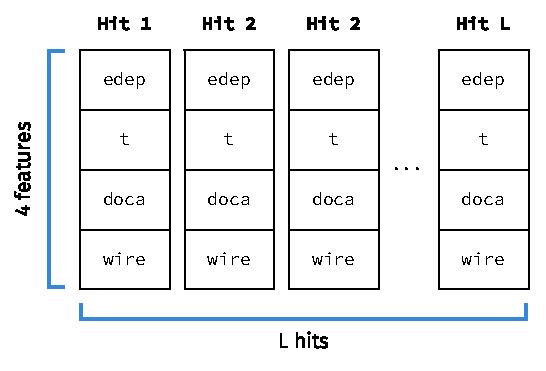
\includegraphics[width=0.5\textwidth]{chapter4/hit_sequence.drawio.pdf}
    \caption{Structure of one training sample. Hits are arranged into
    fixed-length sequences in the {\sc Geant4} order, i.e.\ whereby hits from
    the same track are contiguous.}
    \label{fig:hit_data_structure}
\end{figure}


%In COMET Phase-I, events of particular interest come in the form of extended
% tracks in the CDC, whose accurate reconstruction (in both momentum and
% position) is paramount to the identification of a conversion signal. These
% tracks typically produce hits in very specific patterns, dictated by the
% particle's exact trajectory and energy loss in the gas. We expect a
% data-driven generative model to struggle in replicating the exact signature of
% such tracks, hence we decided early on to restrict the scope of the model to
% events that lack any physics-rich features. ^ not necessarily true. it's not
% only for that reason, but also because we want fine control over the rates of
% specific events (e.g. signal-like)

\subsection{Event selection}

% Consequences: we have to combine MC and GAN data ---> means we have to find a
% way to produce MC selectively ---> and then mix hits in the right proportions
% to get mock data.

Not all MC events are fed to the GAN for training. In particular, potential
background sources, i.e.\ particles with a momentum around
\SI{105}{MeV/\clight}, produce characteristic series of hits in the CDC which
are likely to be reconstructed by a track fitting algorithm. Such a particle's
trajectory is firmly dictated by the Lorentz force, which is a constraint
difficult to impose on a GAN model. In addition, a GAN might generate too large
or too small a proportion of reconstructible events, leading to more uncertainty
in the background rates estimated from samples containing synthetic hits. Unlike
MC data, fake tracks can yield no information concerning their origin, as the
GAN-generated hits come completely unlabelled.

These reasons motivate a splitting of the dataset into \emph{reconstructible}
events, which only the MC simulation may simulate, and \emph{noise-like} events,
where no reconstructible track occurs and the data is deemed ``uninteresting''
enough that it can be augmented by the GAN without biasing the physical results.

% EVENT RECOMBINATION Once the GAN model is trained, it should be able to
%efficiently generate noise-like hits which must then be mixed back into
%MC-simulated reconstructible events in the right proportions. Because the
%generative neural network can leverage parallel processing and GPUs, noise-like
%data is expected to be cheap to produce, hence the bottleneck remains with the
%MC simulation. However the yield of reconstructible events may be increased
%with selective event sampling. 

In each MC event (corresponding to the outcomes of one proton-on-target
collision), we determine if at least one particle with $p >
\SI{50}{\MeV/\clight}$ has entered the CDC and produced at least 4 hits. In this
case, all hits from the event are given the ``reconstructible'' label and will
not be used to train the GAN. If no reconstructible track has occurred during
the event, all hits are considered noise-like and are added to the training
dataset. Figure~\ref{fig:cdc_rconst_vs_noise} compares noise-like and
reconstructible hits and outlines the difference in structure between the two
categories.

\begin{figure}
    \centering
    \captionsetup[subfigure]{justification=centering}
    \begin{subfigure}[t]{0.45\textwidth}
        \centering
        \hspace{-1cm} % To align graphics with caption
        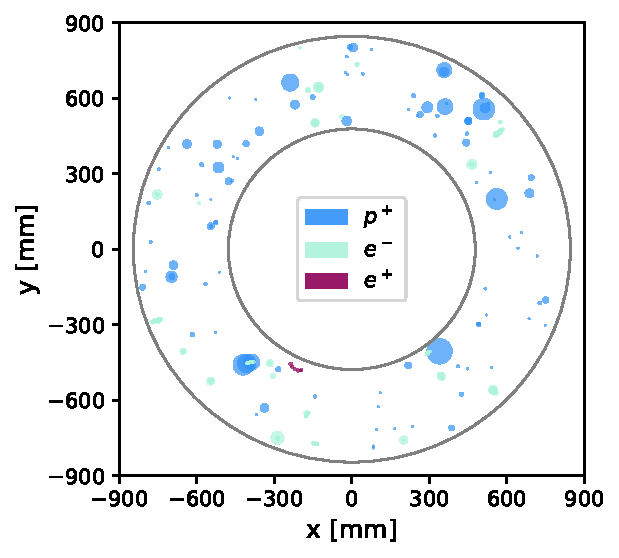
\includegraphics[width=\textwidth]{chapter4/only_noiselike_events.pdf}
        \caption{Noise-like hits from 100 MC events.}
        \label{fig:cdc_rconst_vs_noise:low}
    \end{subfigure}
    \begin{subfigure}[t]{0.45\textwidth}
        \centering
        \hspace{-1cm} % To align graphics with caption
        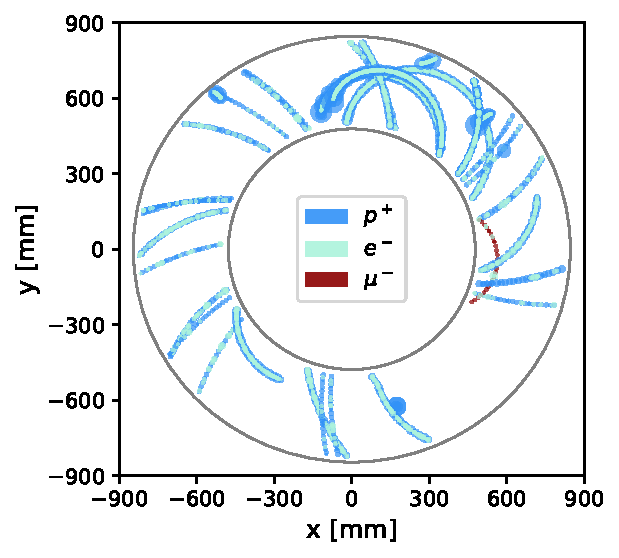
\includegraphics[width=\textwidth]{chapter4/only_reconstructible_events.pdf}
        \caption{Reconstructible hits from 10 MC events.}
        \label{fig:cdc_rconst_vs_noise:high}
    \end{subfigure}
    \caption{Comparison of hit patterns in the CDC depending on whether or not a reconstructible track occurred. The area of each hit is proportional to the amount of energy deposited, and the colour denotes particle type.}
    \label{fig:cdc_rconst_vs_noise}
\end{figure}

The MC5 dataset contains $10^{9}$ events of which \numprint{51137} have hits in
the CDC. Of those, \numprint{2036} events have at least one reconstructible track, and
\numprint{49101} events do not. Inside this latter category, \numprint{634266} hits are
present, and these make up the GAN training dataset.

% MC5A02 calculation of noise-like vs reconstructible events/hits: Total events:
% 990678399 Hit classification: 2036 unique events (rate 2e-6) with
% reconstructible hits (63648 hits) 49101 unique events (rate 5e-5) with
% noiselike hits (634266 hits)



%In order to preserve the information present in events where signal-like tracks
%occur,  MC events are split into two categories, depending on whether or not at
%least one \emph{reconstructible} track appeared in the CDC during the event.
%The GAN is only trained on noise-like hits, while simulating reconstructible
%events is reserved to the Monte Carlo simulation, such that all reconstructed
%tracks have a history which can be retraced all the way to the proton
%collision. This effectively prevents the GAN from producing fake signal-like
%tracks unconstrained, which could cause excessive uncertainties in the
%estimated background rates. However, the two categories of events must now be
%produced separately and later recombined in the right proportions, which adds
%some complexity to the task.

%Training the GAN to generate individual hits is sufficient to model the
%underlying distributions of the four features, but the generated hits lack
%coherence. In the training dataset, when multiple hits are produced by a single
%track, they often occur next to each other in time and space. The GAN model
%must be allowed to see and process the relationship between consecutive hits
%for the generated hits to resemble simulated ones. Hence instead of having the
%model process single hits, it makes sense to feed it sequences of consecutive
%hits such that temporal information can be processed as well. The architecture
%of $G$ and $D$ should be allowed to accommodate for this extra dimension.


% This is what hits from p>50MeV tracks look like, and this is what hits from
% p<50MeV tracks look like. From the observation that the former tends to have
% reconstructible hit patterns while the latter contains single hits and
% localised patterns, we categorise MC events according to whether they contain
% a p>50MeV track or not. We then use hits from non-reconstructible events as
% the training data for our generative model whose goal is to learn the patterns
% and generate original samples of hits that we can use as a background onto
% which we will overlay reconstructible MC-simulated events. The result is the
% offloading of 99% of the simulation to the generative model which is highly
% efficient. 



\subsection{Pre-processing}
The three continuous hit features (energy deposit, time and DCA) are physical
quantities with different units and scales. Their distributions are shown in
Figure~\ref{fig:original_feature_distributions}. In order to maximise gradient
flow in the discriminator, it is common practice for all features to be
re-scaled into a fixed range, e.g.\ $[0, 1]$. However, in the case of highly
uneven and/or discontinuous distributions, the generator can struggle to model
the data which results in a distribution of generated data which does not match
the distribution of training data.

\begin{figure}
    \centering
    \noindent\makebox[\linewidth][c]{
        \begin{subfigure}[t]{0.35\textwidth}
            \centering
            \hspace{-0.5cm}
            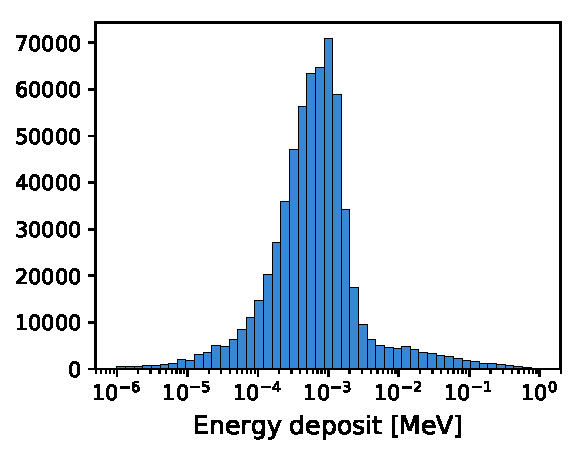
\includegraphics[width=\textwidth]{chapter4/real_edep.pdf}
            %\caption{}
        \end{subfigure}
        \begin{subfigure}[t]{0.35\textwidth}
            \centering
            \hspace{-0.5cm}
            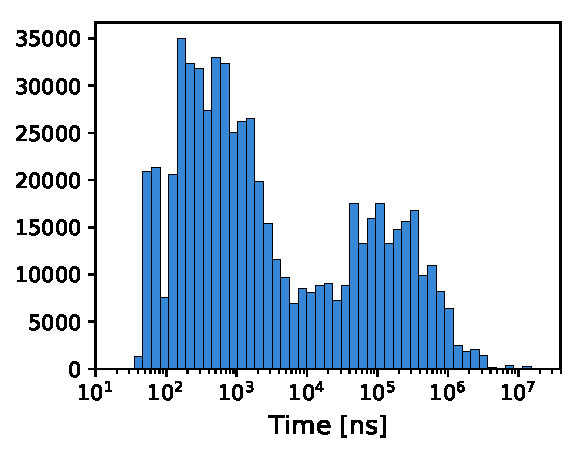
\includegraphics[width=\textwidth]{chapter4/real_t.pdf}
            %\caption{}
        \end{subfigure}
        \begin{subfigure}[t]{0.35\textwidth}
            \centering
            \hspace{-0.5cm}
            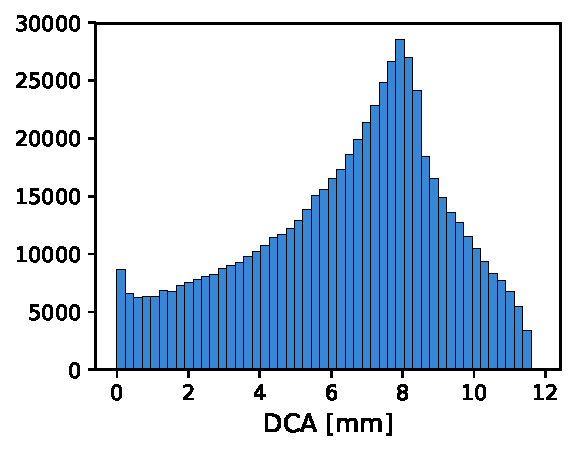
\includegraphics[width=\textwidth]{chapter4/real_doca.pdf}
            %\caption{}
        \end{subfigure}}
    \caption{Distributions of the three continuous features used to train the GAN.}
    \label{fig:original_feature_distributions}
\end{figure}

To alleviate this issue and define a common scale for all continuous features,
each feature undergoes a non-linear \emph{quantile transformation}, which
corresponds to a mapping from each value $x_i$ to $y_i = \Phi^{-1}(F(x_i))$,
where $F$ is the empirical cumulative distribution function (CDF) of the
feature, and $\Phi$ is the Gaussian CDF. This transformation effectively yields
normally distributed features, which the generator can more easily reproduce.
Its task is not however made trivial, as the correlations between features
remain, which it must learn to model.

In addition to the quantile transformation, the values of each feature are
re-scaled independently to lie within the $[-1, 1]$ range. To prevent the
generator from producing values out of this range, which would give the
discriminator a clear indication of a sample being fake, the hyperbolic tangent
function is used as the generator's final layer.

%We use the standard classes \texttt{preprocessing.QuantileTransformer} and
%\texttt{preprocessing.MinMaxScaler} from the Scikit-learn~\cite{sklearn}
%package to apply these pre-processing steps.

%The fourth feature, wire index, is not modified prior to training. However, as
% the only discrete quantity, it receives a special treatment by the networks
% during training. More? Less?

\subsection{Hit sequence sampling and data augmentation}
At each step of the training, the discriminator receives two mini-batches of hit
sequences: one from the training data and one synthesised by the generator. The
discriminator's output is then used to compute the loss for $G$ and $D$,
according to Eqs.~\ref{eq:WGAN-GP} and~\ref{eq:WGAN-GP_gen}.

To allow parallel processing of the hit sequences by the networks, a fixed
sequence length $L$ is defined prior to training. Hence hits can be packed
into dense tensors upon which vectorised operations can be applied. Typically, a
sequence will contain concatenated sets of hits from multiple tracks and from
multiple events.

Hits belonging to different events are completely unrelated, as they are not the
product of the same POT collision. This provides freedom to swap events and
concatenate their hits in any order. The order of hits within the same event
should however be preserved. 
Combining events in many different ways enhances the diversity and size of the
training dataset, which alleviates the possibility of overfit or mode collapse.
Concatenating the \numprint{634266} hits linearly into sequences of length
$L=512$ would yield only 1239 samples. By rearranging the events, we produce
\numprint{500000} unique samples which the GAN learns from. Although it is not
the maximum number of event re-combinations, this number of samples was found to
be large enough to prevent overfit of our GAN model.


\subsection{Network components}

\subsubsection{Temporal convolutions}
In order to process sequences of hits efficiently, both networks use a series of
convolutional layers which --- unintuitively --- apply cross-correlation
operations between the input $x$ and the learned kernel $w$:
\begin{equation}\label{eq:conv1d}
    %y_{i} = (x \ast w)_{i} + b = \sum_{j=1}^{C_\mathrm{in}} \sum_{k=-(K-1)/2}^{(K-1)/2} w_k\ x_{i+k,j} + b,
    y_{i} = (w \ast x)_{i} = \sum_{k} w_k \cdot x_{i+k},
\end{equation}
where $i$ is the position along the output sequence $y$, and $k$ runs over the
kernel weights. This operation is illustrated in Figure~\ref{fig:temporal_conv}.

\begin{figure}
    \centering
    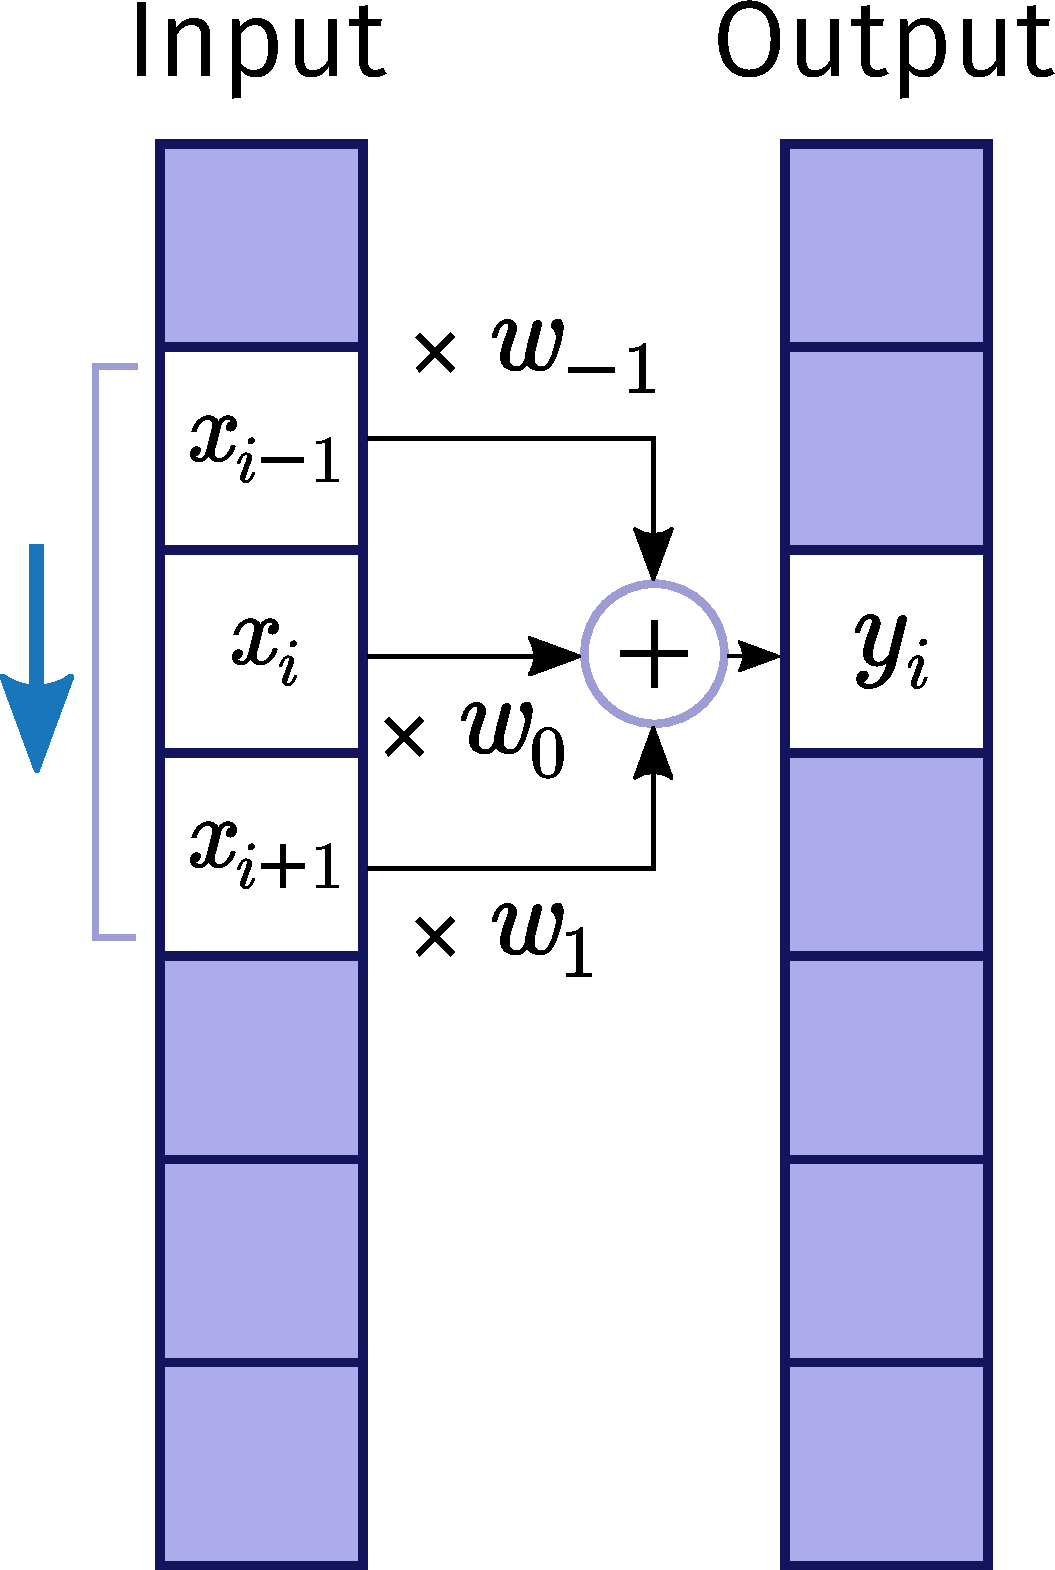
\includegraphics[width=0.20\textwidth]{chapter4/1d_convolution.pdf}
    \caption{Temporal (1D) convolution operation with kernel size 3. For
    clarity, both the input and output sequences have one channel, i.e.\
    $C_\mathrm{in} = C_\mathrm{out} = 1$. The blue arrow shows the direction along
    which the kernel slides across the input sequence.}
    \label{fig:temporal_conv}
\end{figure}


Unlike in the common case of raster images, the input to the discriminator is
not a two-dimensional array of pixels, but a one-dimensional sequence of hits.
Hence the kernels are also one dimensional. The ``channels'' of the input
sequence correspond to features of the hits. Within a convolutional layer,
Eq.~\ref{eq:conv1d} is applied as many times as there are channels in the input
sequence, and the result is the sum over channels. The operation can also be
applied in parallel with many different kernels, in which case each kernel will
produce one channel in the output sequence.


The fact that the kernel acts on adjacent elements implies that the network
effectively processes multiple consecutive hits at a time. This allows the
generator to synthesise coherent sequences and the discriminator to perceive
whether a generated sequence has the same overarching structure as real
sequences.

%\subsubsection{Strided convolutions for up- and down-sampling}
Optionally, convolution kernels can be applied over the sequence with a stride,
meaning that the kernel moves down by more than one element between two
cross-correlation operations. This has the effect of producing an output
sequence that is shorter than the input sequence. This is often used to allow
the network to see the data over increasingly large scales and to keep the total
number of operations reasonable in layers where the input has many channels.

%In the generator, fractionally-strided convolutions are used in order for the
%sequence length to increase


%The discriminator takes as input a sequence of hits of length $L$. Each hit is
%described by four features: energy deposit, time, distance of closest approach
%and wire index. The first convolutional layer computes feature maps by sliding
%its kernels over the hit sequence. A non-linear activation function is applied
%to the feature maps before passing them on to the next layer. In our case, the
%leaky rectified linear unit, or
%\texttt{LeakyReLU}~\cite{Maas13rectifiernonlinearities}, is used as the
%non-linearity. ^ Too much detail?


\subsubsection{Residual connections}
\begin{figure}
    \centering
    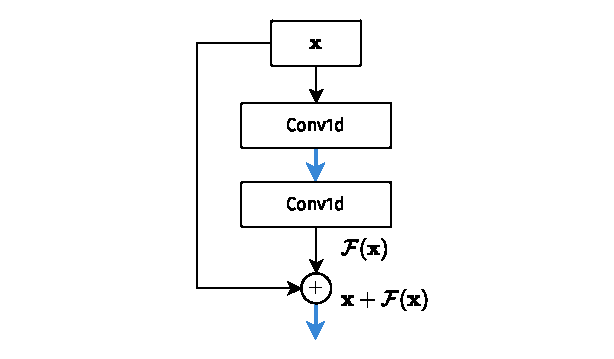
\includegraphics[width=0.6\textwidth]{chapter4/residual_sel.drawio.pdf}
    \caption{Residual blocks used in both networks to facilitate gradient flow.
    Blue arrows indicate an activation function.}
    \label{fig:residual_block}
\end{figure}
In order to facilitate gradient flow from the discriminator to the generator and
thus speed up training, convolutional layers can be replaced by residual
blocks~\cite{he2016deep} in both networks. A residual block combines two
convolutional layers with a residual connection from the input to the output,
allowing the gradients to propagate via two paths, as shown in
Figure~\ref{fig:residual_block}. The output $\bm{y}$ of the block can be
written as
%\begin{equation*}
    $\bm{y} = \mathcal{F}(\bm{x}) + \bm{x},$
    %\bm{y} = \mathcal{F}(\bm{x}) + W_s \bm{x},
%\end{equation*}
where $\mathcal{F}$ represents the operation of the two convolutional layers and
$\bm{x}$ is the input tensor. 
When $\mathcal{F}(\bm{x})$ and $\bm{x}$ have different shapes, a
dimension-matching linear transformation can be applied to $\bm{x}$. In this
case, the result is $\bm{y} = \mathcal{F}(\bm{x}) + W \bm{x}$, where the
weights of the $W$ tensor are adjusted during training.


\subsection{Network architectures}
Having introduced the building blocks, we can now assemble them into our
discriminator and generator. The two networks, shown schematically in
Figure~\ref{fig:architectures}, are composed of stacked residual blocks, which
progressively increase the size of the sequence in the generator, or decrease it
in the discriminator.

\begin{figure}
    \centering
    \begin{subfigure}[t]{0.49\textwidth}
        \centering
        \caption{Generator.}
        \vspace{0.3cm}
        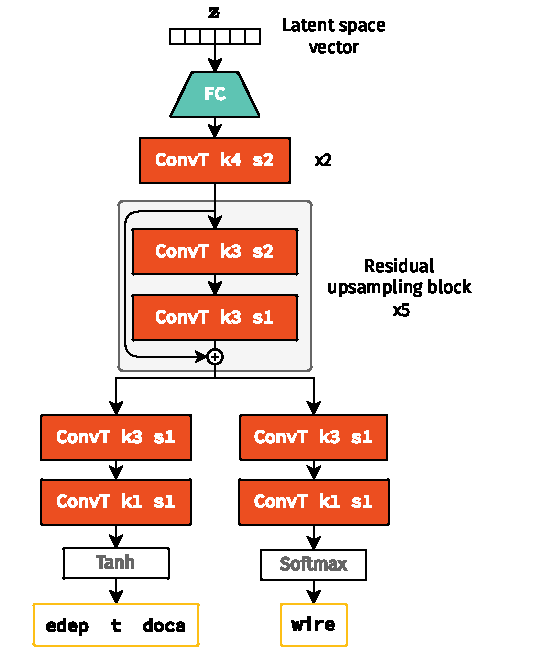
\includegraphics[width=\textwidth]{chapter4/network_architectures_gen.drawio.pdf}
        \hspace{-1cm} % To align graphics with caption
    \end{subfigure}
    \\
    \vspace{0.5cm}
    \begin{subfigure}[t]{0.49\textwidth}
        \centering
        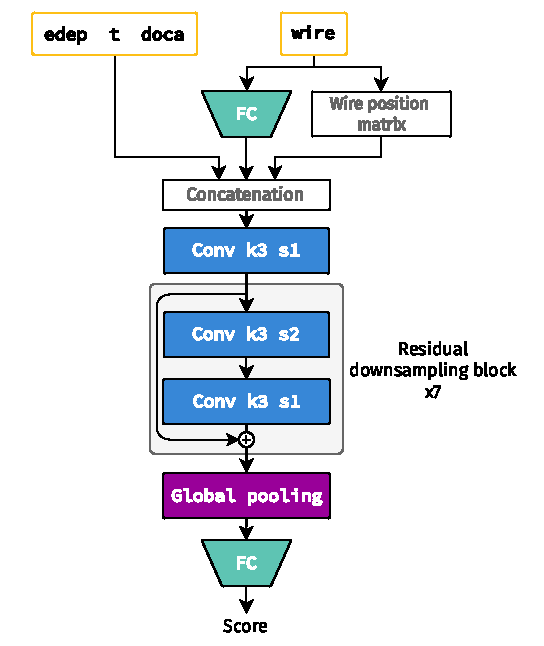
\includegraphics[width=\textwidth]{chapter4/network_architectures_disc.drawio.pdf}
        \hspace{-1cm} % To align graphics with caption
        \caption{Discriminator.}
    \end{subfigure}
    \caption{Network architectures. The layer types are: \texttt{FC} for
        fully-connected, \texttt{Conv} for a standard convolution and
        \texttt{ConvT} for a transposed (fractionally-strided) convolution. In
        convolutional layers, kernel size and stride are denoted by \texttt{k}
        and \texttt{s}, respectively.}
    \label{fig:architectures}
\end{figure}

\subsubsection{Data flow}
In the generator, the input vector, sampled from latent space, is first passed
through a fully-connected layer, after which it is reshaped to have a length of
4. The proto-sequence is then up-sampled by fractionally-strided convolutional
layers, adding finer and finer details to the sample. As the length increases,
the number of channels is decreased to limit the total number of operations and
the network's complexity. Once the sample has reached a length of $L$, the
information is projected to data space: to obtain the continuous features, a
convolutional layer with three output channels is applied and its output passed
through a $\tanh$ function, yielding values in the range $[-1, 1]$; while for
the discrete wire index, we use a layer with 4986 output channels\footnote{As
many as there are wires.} followed by a softmax\footnote{Defined as
$\mathrm{Softmax}(\bm{x})_i = \frac{\exp(-x_i)}{\sum_j \exp(-x_j)}.$}
function to determine the network's preferred choice of wire for each hit.

The discriminator extracts information from the input hits through its
convolutional layers, progressively down-sampling the sequence while increasing
the number of channels. After 7 residual blocks, a global average pooling is
performed, i.e.\ for each channel, the result is the average value over the
sequence. The resulting tensor is passed through a final fully-connected layer,
combining the features into a single scalar which is the score for that sample.

\subsubsection{Gradient flow for discrete features}
We would like for the discriminator to have some knowledge of where, in the
detector, hits are located, so that it can use this knowledge as a criterion in
its judgement. A straightforward way to give this information to the
discriminator would be to use the wire index to query a lookup table of wire
positions. However, indexing an array is not a differentiable operation, hence
it does not allow gradients to flow from the output score to the generator
weights, and this prevents the generator from learning to accurately position
hits.

To allow gradient flow, we can represent the wire index as a \emph{one-hot
encoded} vector, whose size is the total number of wires, and where only the
entry corresponding to the index is 1, and the others are 0. This vector
representation can be used in differentiable operations to query a particular
entry in a table: if we represent the table of wire positions as a matrix $W$
with dimensions $2 \times 4986$, and the one-hot encoded wire vector as a
4986-dimensional vector $\bm{v}$, the product $W \cdot \bm{v}$ is a
differentiable operation and its output is the wire's position since the one-hot
vector picks out the correct entry from the position matrix.

In the case of generated hits, the wire vector is not exactly one-hot: instead,
the output of the softmax operation is a vector of real-valued probabilities for
each wire. The multiplication of the above wire position matrix with such a
vector can be interpreted as a weighted sum of all wire positions with the
weight corresponding to the softmax probability. Hence the result is not an
exact wire location but an approximate region of the detector in which the
generator envisions the hit to be.

As discussed in~\cite{NIPS2017_892c3b1c}, one might suspect that the
discriminator can learn to reject the output of the generator because it does
not look like a one-hot vector. However the Wasserstein distance between the
real and generated data remains well-defined and continuous even in this
particular case of a discrete variable, hence using the WGAN loss does allow the
networks to learn.


\subsection{Training}
The networks are trained via gradient descent of the WGAN-GP loss, using the
Adam~\cite{Kingma2015AdamAM} algorithm. The PyTorch framework with which the GAN
is implemented allows all tensor operations to be performed on a Nvidia Graphics
Processing Unit (GPU) via CUDA, which speeds up training iterations roughly
tenfold. Hyperparameters, such as learning rate and $\lambda_{GP}$, were
initially set to a default value from common practice guidelines and then
adjusted if needed to ensure stable loss curves.
Table~\ref{tab:training_hyperparameters} summarises the values of various
hyperparameters, and Figure~\ref{fig:gan_losses} shows the loss curves for $G$
and $D$ over 200 training epochs.

\begin{table}[]
    \centering
    \begin{tabular}{cccccc}
        \toprule
        Optimiser & Learning rate & $(\beta_1, \beta_2)$ & Sequence length & Loss &
        $\lambda_\mathrm{GP}$
        \\\midrule 
        Adam & $10^{-4}$ & $(0.9, 0.999)$ & 512 & WGAN-GP & 10
        \\\bottomrule
    \end{tabular}
    \caption{Training hyperparameters.}
    \label{tab:training_hyperparameters}
\end{table}

The loss functions for $D$ and $G$ evaluated at each training step are recorded
to show the progression and ensure that the networks are learning. In addition,
every 100 mini-batch iterations, the critic loss is evaluated on test samples
which are absent from the training dataset. This allows us to determine whether
$D$ is overfitting to the training data, in which case the loss calculated using
training and test samples (Figure~\ref{fig:gan_losses:test}) would diverge, as
demonstrated in~\cite{NIPS2017_892c3b1c}.


\begin{figure}
    \centering
    \begin{subfigure}{0.49\textwidth}
        \centering
        \hspace{-1cm} % alignment
        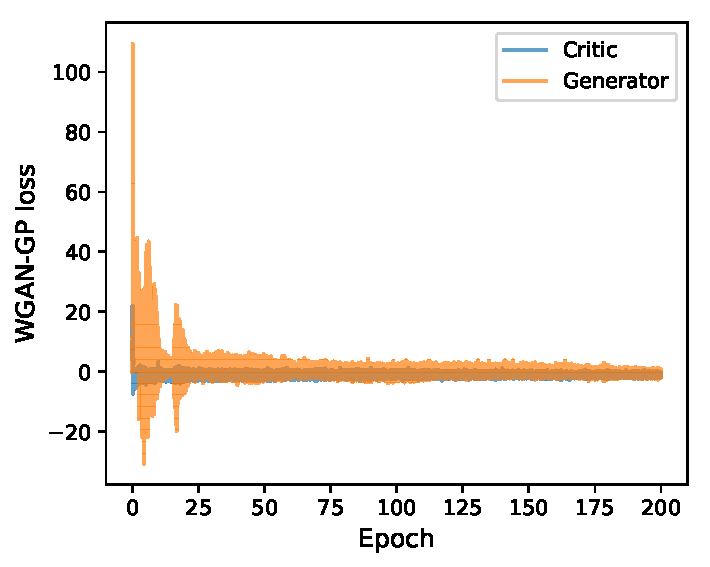
\includegraphics[width=0.95\textwidth]{chapter4/losses.pdf}
        \caption{Critic and generator losses.}
    \end{subfigure}
    \hfill
    \begin{subfigure}{0.49\textwidth}
        \centering
        \hspace{-1cm} % alignment
        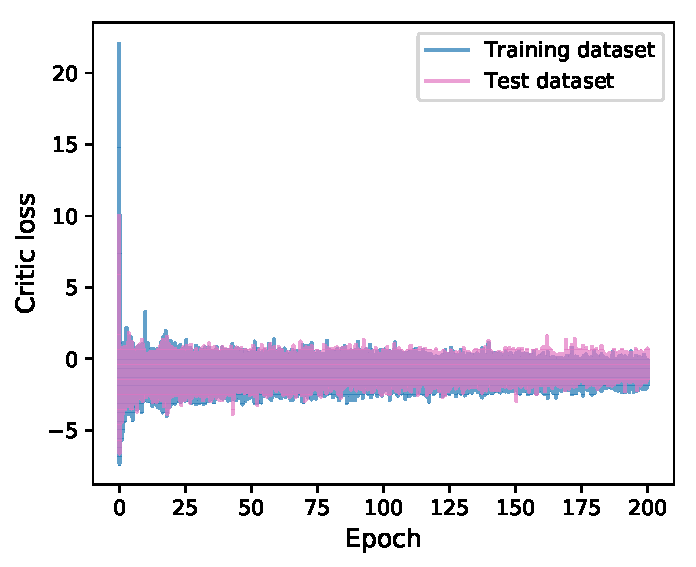
\includegraphics[width=0.95\textwidth]{chapter4/val_loss.pdf}
        \caption{Critic loss for training and test samples.}
        \label{fig:gan_losses:test}
    \end{subfigure}
    \caption{Loss curves as a function of training epochs.}
    \label{fig:gan_losses}
\end{figure}

% Weight initialisation def weight_init_gen(m): classname = m.__class__.__name__
% if classname.find('Conv') != -1: nn.init.normal_(m.weight, 0.0, 0.02) if
% m.bias is not None: nn.init.zeros_(m.bias)

% def weight_init_disc(m): classname = m.__class__.__name__ if
%     classname.find('Conv') != -1: nn.init.normal_(m.weight, 0.0, 0.02) if
%     m.bias is not None: nn.init.zeros_(m.bias) if classname.find('Linear') !=
%     -1: nn.init.normal_(m.weight, 0.0, 0.02) if m.bias is not None:
%     nn.init.zeros_(m.bias)



\subsection{Evaluation}
\label{sec:gan_eval}
Evaluation of GAN-generated samples is notoriously difficult in all domains
because of the lack of a well-defined, unique metric for quality\footnote{Unlike
in supervised learning, where an obvious quality metric is usually the loss
function itself.}. The score
returned by the discriminator network is dependent upon its exact architecture,
the dataset and all hyperparameters, hence it cannot be used as a reliable metric. 

Unlike natural images which can be examined visually to determine whether or not
they depict something real, sequences of hits in a detector are difficult to
evaluate perceptually. 
Figure~\ref{fig:comp_uncurated} shows a comparison between uncurated individual
samples, four from the training dataset and four generated by $G$. In this type
of evaluation, we try to exacerbate any differences in the features and
sequence structure through colours and visual hints such as lines connecting
consecutive hits.

On a larger scale, we also compare the distributions of hit features across many
samples in order to verify that the GAN can model the dataset properly. Drawing
2D histograms of each pair of feature, as in
Figure~\ref{fig:comp_feature_distributions}, also reveals whether or not feature
correlations are faithfully modelled by $G$.

\begin{figure}
    \centering
    \captionsetup[subfigure]{justification=centering}
    \begin{subfigure}[t]{0.48\textwidth}
        \centering
        \hspace{-1cm} % To align graphics with caption
        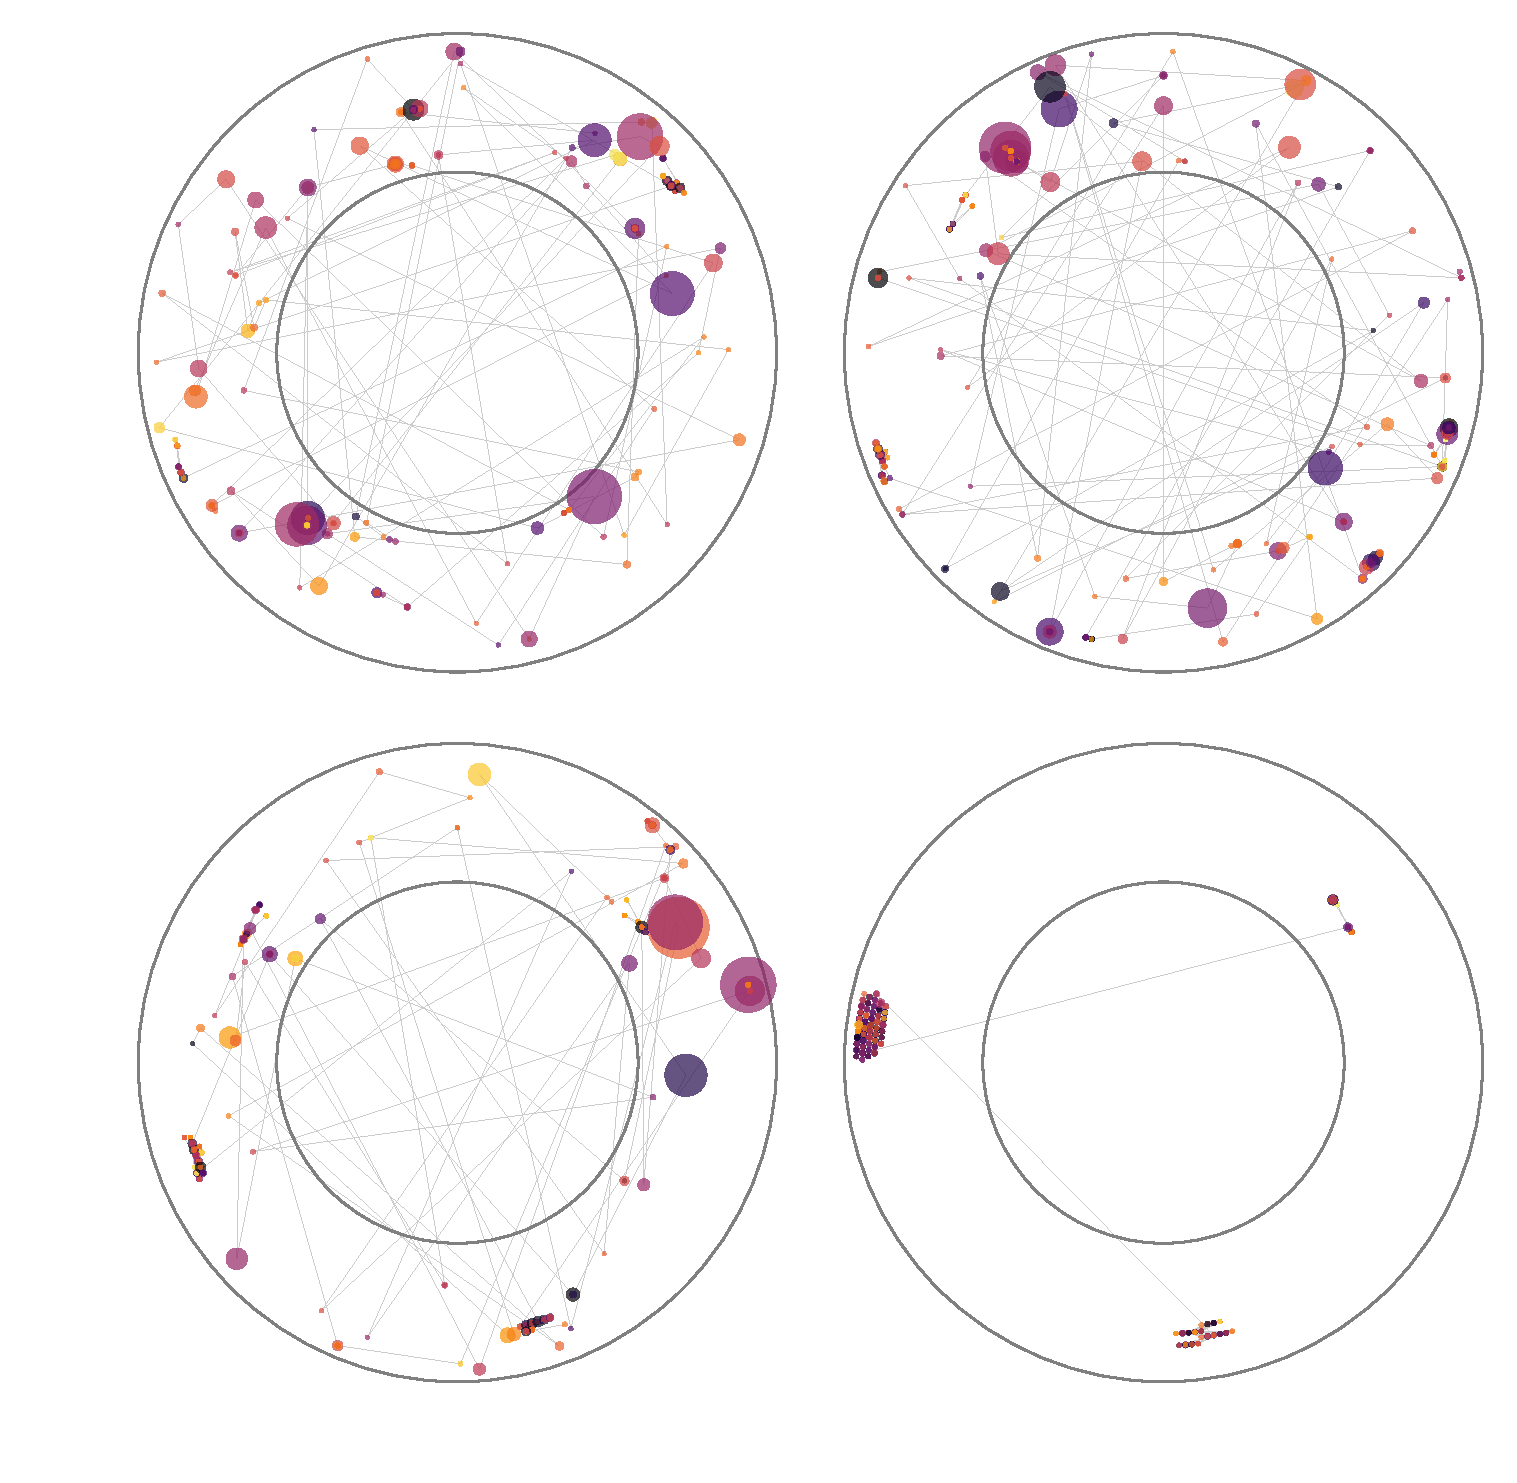
\includegraphics[width=\textwidth]{chapter4/grid_real_4.pdf}
        \caption{Training samples.}
    \end{subfigure}
    \quad
    \begin{subfigure}[t]{0.48\textwidth}
        \centering
        \hspace{-1cm} % To align graphics with caption
        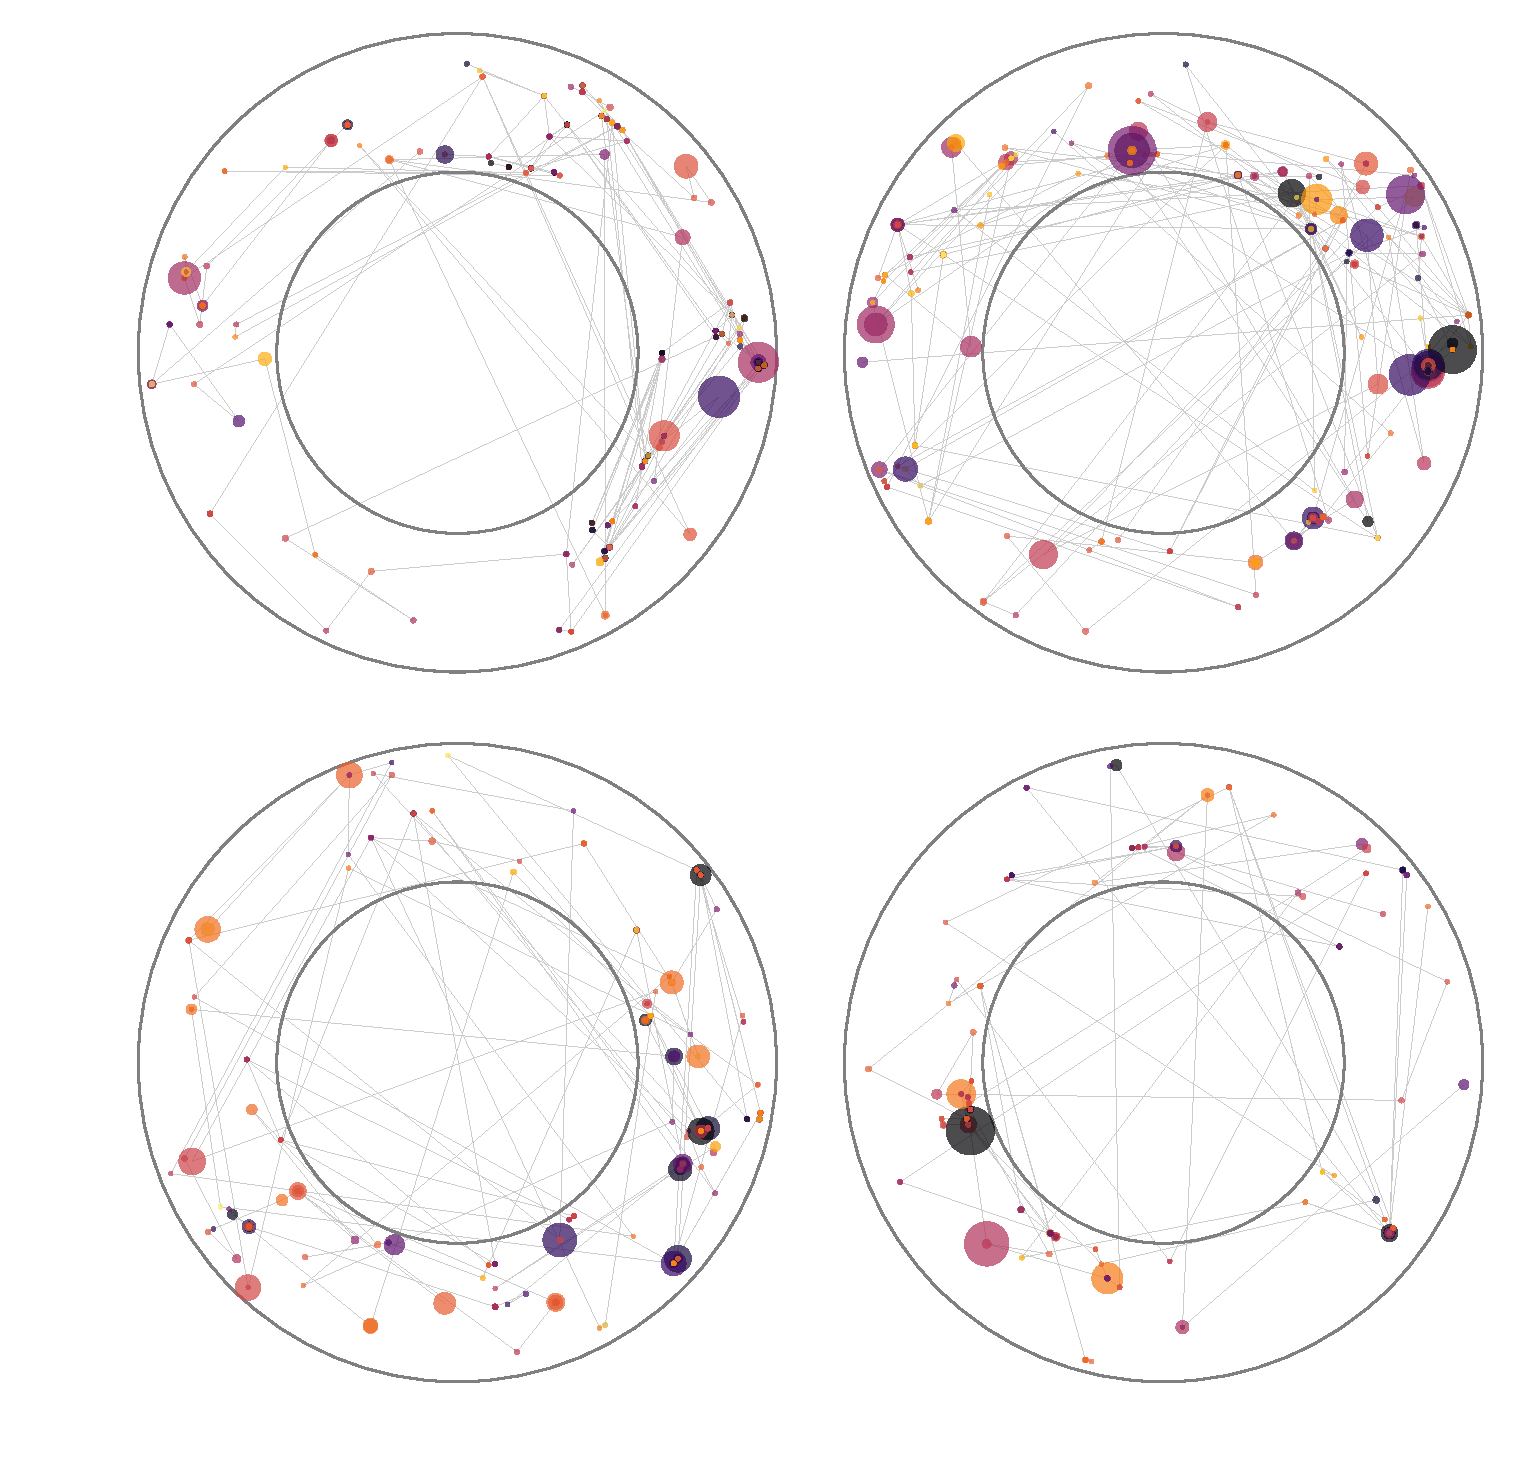
\includegraphics[width=\textwidth]{chapter4/grid_fake_4.pdf}
        \caption{Generated samples.}
    \end{subfigure}
    \caption{
        Comparison of individual samples, comprised of 512 hits. Hits are
        represented by a circle whose area is proportional to the energy deposit
        and whose colour shows distance of closest approach. 
        Lines connect consecutive hits in the sequence.
        %Only three features out of four can be examined and compared using
        %these plots unless we add an extra dimension.
    }
    \label{fig:comp_uncurated}
\end{figure}

\begin{figure}
    \centering
    \captionsetup[subfigure]{justification=centering}
    \begin{subfigure}[t]{0.48\textwidth}
        \centering
        \hspace{-1cm} % To align graphics with caption
        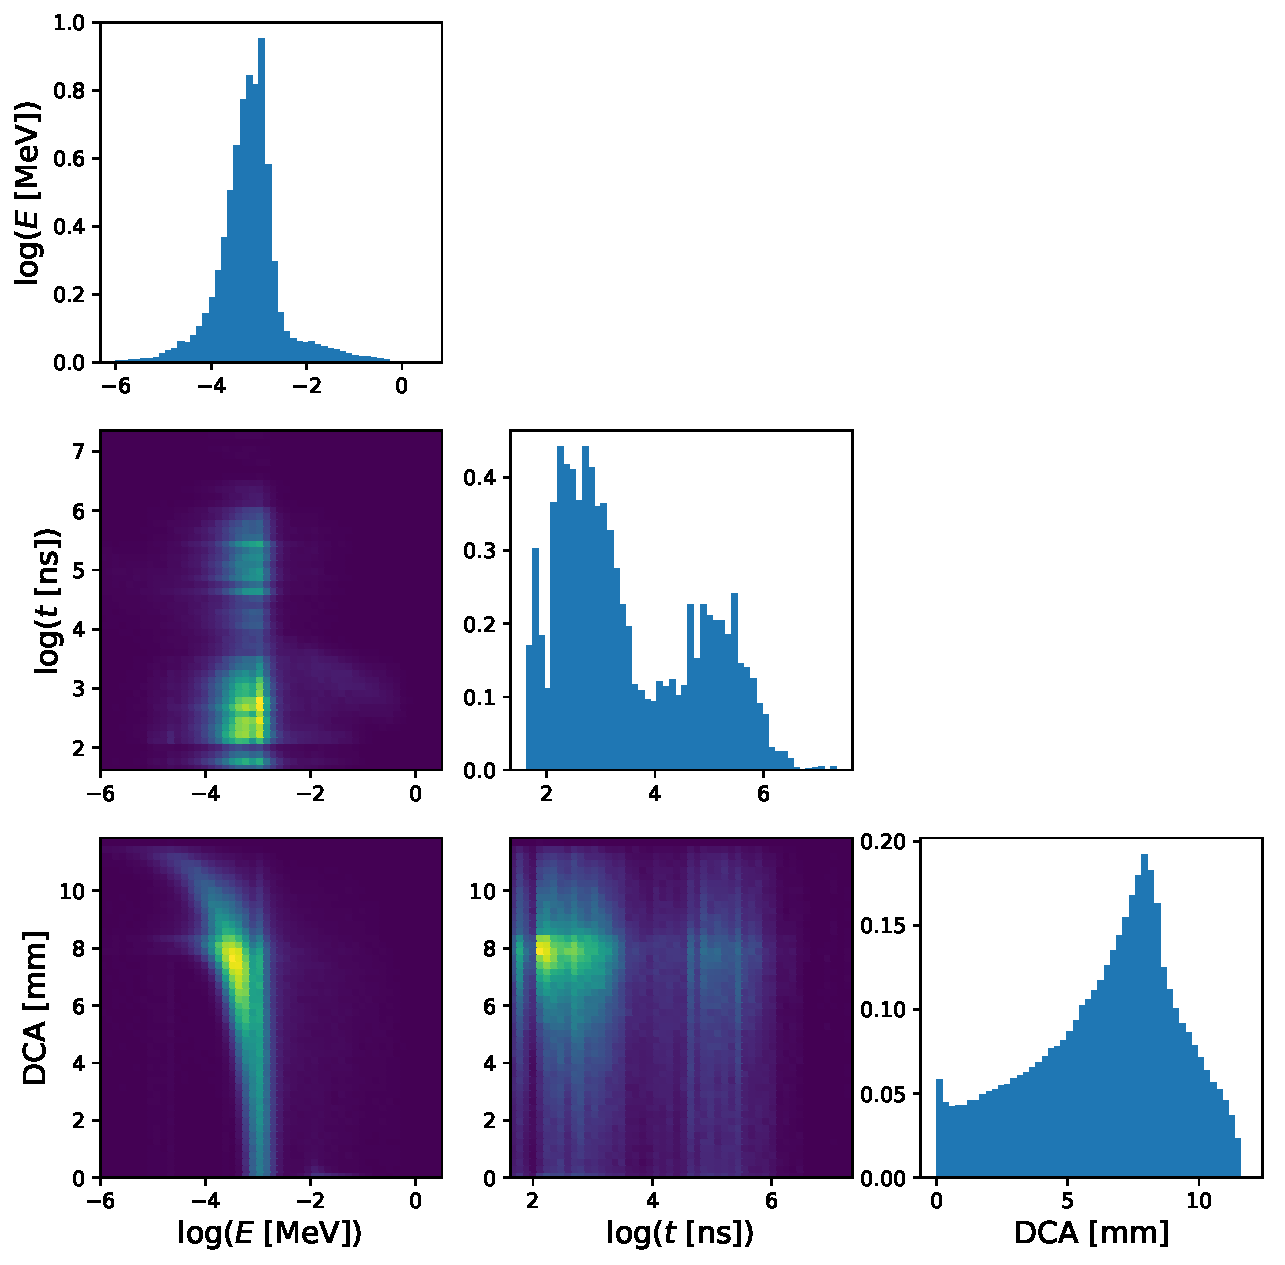
\includegraphics[width=\textwidth]{chapter4/feature_matrix_real.pdf}
        \caption{Training dataset.}
    \end{subfigure}
    \quad
    \begin{subfigure}[t]{0.48\textwidth}
        \centering
        \hspace{-1cm} % To align graphics with caption
        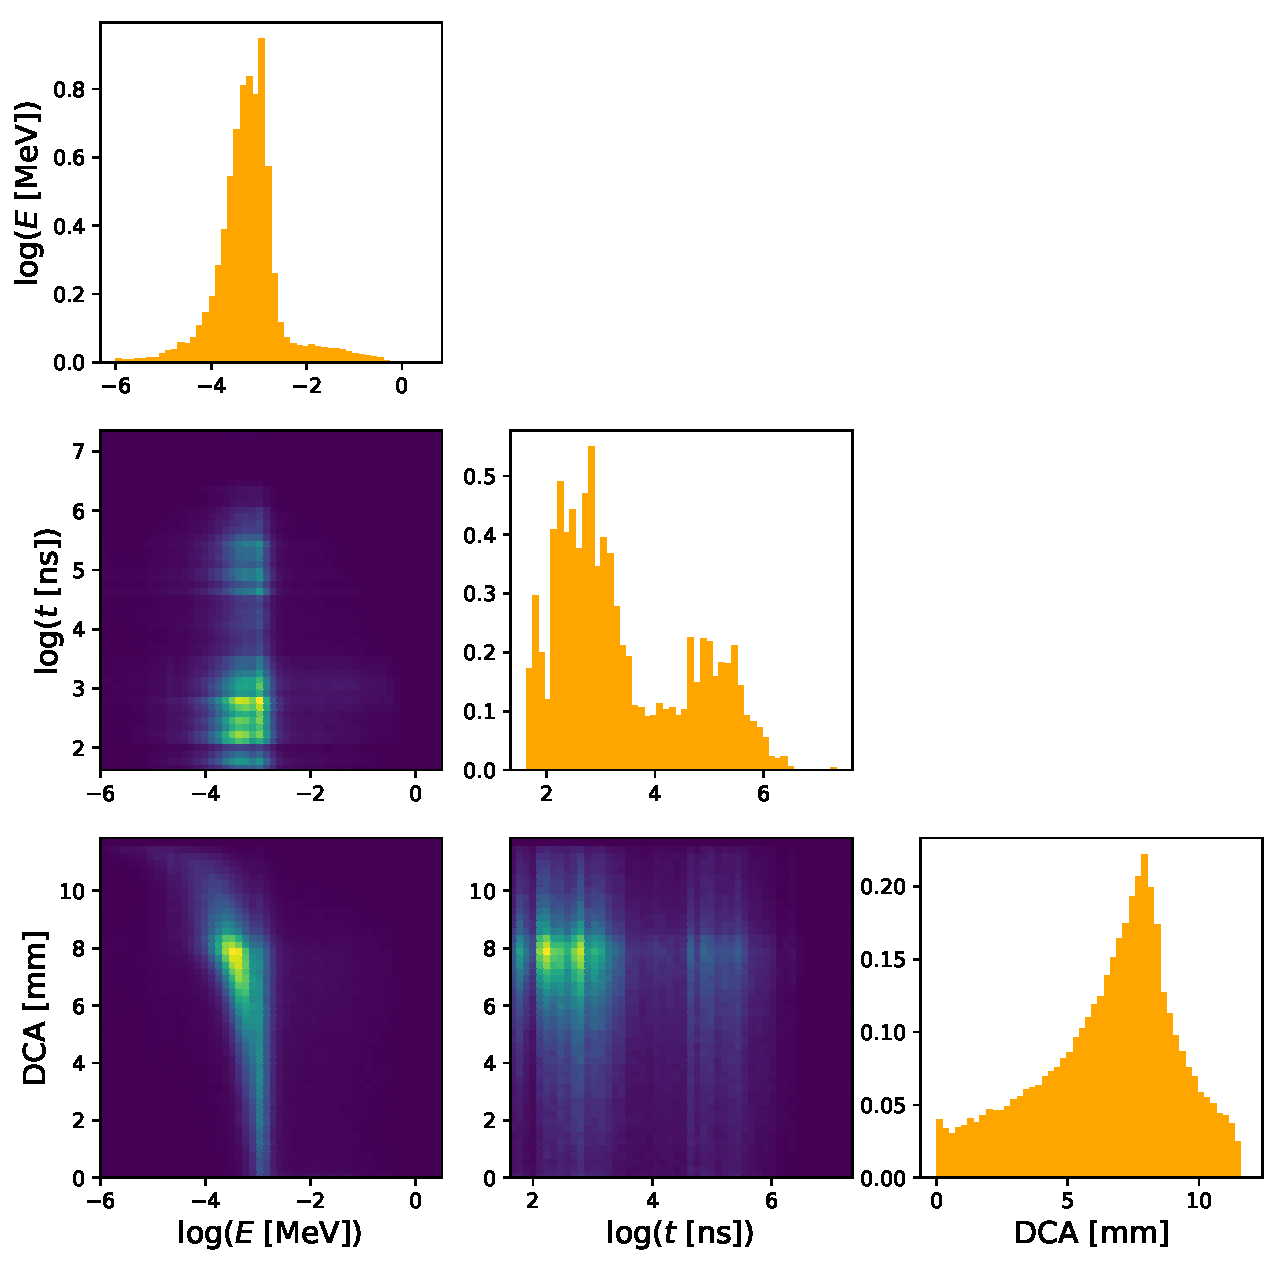
\includegraphics[width=\textwidth]{chapter4/feature_matrix_fake.pdf}
        \caption{GAN-generated dataset.}
    \end{subfigure}
    \caption{
        Comparison of feature distributions and correlations when generating a
        dataset of the same size as the training dataset.
    }
    \label{fig:comp_feature_distributions}
\end{figure}

% For KL div (P || Q) notation
\DeclarePairedDelimiterX{\infdivx}[2]{(}{)}{%
  #1\;\delimsize\|\;#2%
}


In order to summarise the similarity between the distribution of real and generated
samples into one quantity, a commonly used metric is the Kullback-Leibler (KL)
divergence which can be interpreted as the amount of information lost when
approximating the real dataset with the generated one~\cite{10.1214/aoms/1177729694}.
KL divergence is defined on a probability space $\mathcal{X}$ as
\begin{equation}\label{eq:kl_div}
D_\mathrm{KL} \infdivx{P}{Q} = \sum_{x \in \mathcal{X}} P(x) \log \frac{P(x)}{Q(x)},
\end{equation}
where in our case $P$ denotes the distribution of real hits and $Q$ that of
generated hits. To compute $D_\mathrm{KL}$, the three continuous features of
every hit are binned into a 3D histogram to approximate the probability density
functions $P$ and $Q$ and the sum in Eq.~\ref{eq:kl_div} is a sum over all
(non-zero) bins. The \texttt{edep} and \texttt{t} features are log-transformed
such that the resulting histogram is smoother. Figure~\ref{fig:kl_div} shows the
Kullback-Leibler divergence between the continuous distributions of real and
generated hits over training iterations. For this specific model, the KL
divergence converges around 100 epochs.


\begin{figure}
    \centering
    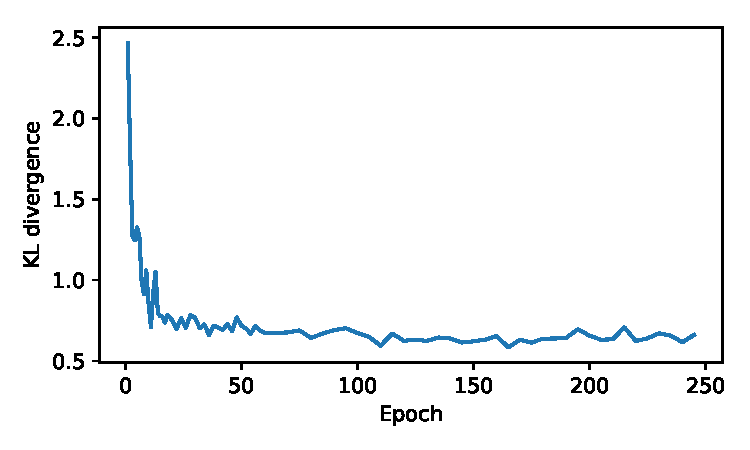
\includegraphics[width=0.5\textwidth]{chapter4/job_21175015_kldiv.pdf}
    \caption{Kullback-Leibler divergence between the distributions of real and generated hits as a function of training epochs.}
    \label{fig:kl_div}
\end{figure}

In addition to comparing the features that are given as input to the GAN for
training, we also examine quantities which are only present implicitly in the
training samples. Figure~\ref{fig:comp_nonlearned} shows a
comparison of the relative amounts of hits in each CDC layer and of the
``occupancy'' per sample, i.e.\ the fraction of wires on which a hit occurs.
This allows us to determine whether or not the model sees beyond the features
provided explicitly for training.

\begin{figure}
    \centering
    \captionsetup[subfigure]{justification=centering}
    \begin{subfigure}[t]{0.38\textwidth}
        \centering
        \hspace{-1cm} % To align graphics with caption
        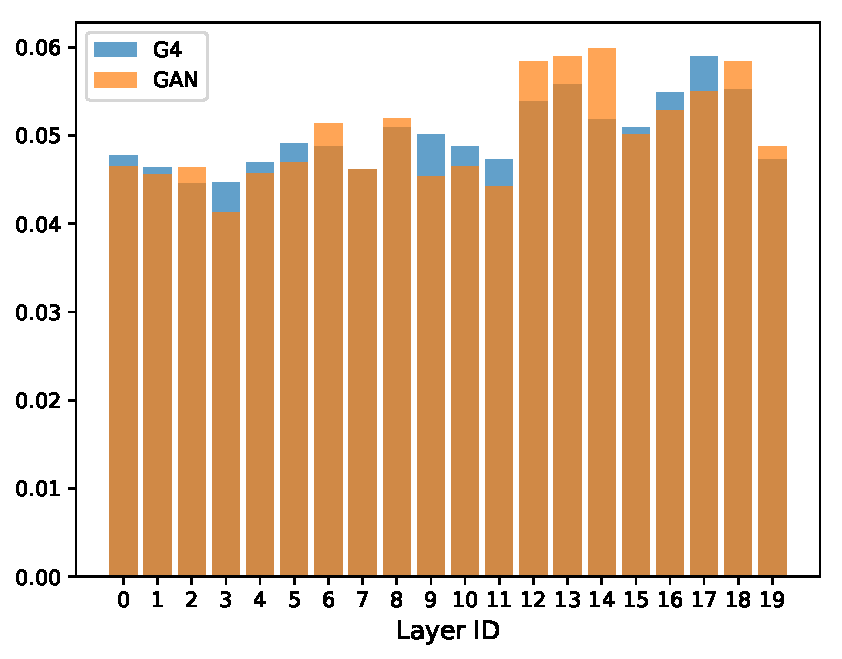
\includegraphics[width=\textwidth]{chapter4/comp_layer.pdf}
        %\caption{Training dataset.}
    \end{subfigure}
    \hspace{2cm}
    \begin{subfigure}[t]{0.38\textwidth}
        \centering
        \hspace{-1cm} % To align graphics with caption
        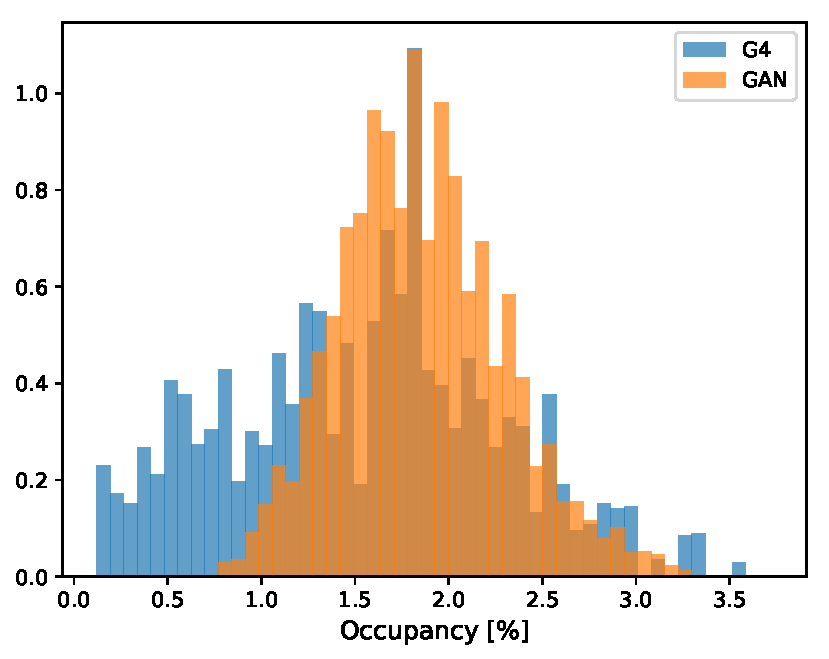
\includegraphics[width=\textwidth]{chapter4/occupancy.pdf}
        %\caption{GAN-generated dataset.}
    \end{subfigure}
    \caption{
        Comparison of quantities not explicitly learned by the GAN model.
    }
    \label{fig:comp_nonlearned}
\end{figure}


\subsection{Quality metrics}\label{sec:quality_metrics} % FID, custom CNN, transfer learning w/ Inception-v3
%In comparing images generated by different GAN models, 
In image generation tasks, the \emph{Inception score} was proposed as a quality
metric to compare images generated by different GAN
models~\cite{salimans_improved_2016}. 
An Inception model~\cite{7298594}, trained independently on the ImageNet dataset
to classify images, is applied to GAN-generated images to obtain label
probabilities for each sample. The metric is then formulated in terms of the label
distribution to favour generated images which depict a specific object rather than
some average of classes, while disfavouring a generator whose images all resemble
the same class.

% $$
% \mathrm{Inception\ score} = \exp \mathrm{KL}(p(y|x)\ ||\ p(y)),
% $$
% where $\mathrm{KL}$ denotes the Kullback-Leibler divergence, $p(y|x)$ is the
% distribution of label probabilities assigned by the Inception network, and
% $p(y)$ is the marginal $p(y) = \int p(y|x = G(z)) \mathrm{d}z$.

The Fréchet Inception Distance (FID) is an evolution of the Inception score
which additionally uses statistics extracted from the training dataset to
estimate a distance between real and generated
samples~\cite{10.5555/3295222.3295408}. Conventionally, a pretrained Inception
v3 model~\cite{7780677} is applied to real and generated samples. Activations
from an intermediate layer are extracted and their mean $\bm{\mu}$ and
covariance $\bm{\Sigma}$ are estimated, from which the Fréchet (or
Wasserstein-2) distance is calculated as
$$
d^2 = | \bm{\mu}_G - \bm{\mu}_R |^2 + 
    \mathrm{Tr}(\bm{\Sigma}_G + \bm{\Sigma}_R - 
    2(\bm{\Sigma}_G \bm{\Sigma}_R)^{1/2})
$$
where the $G$ and $R$ subscripts respectively denote generated and real statistics.

Applying these methods to domains other than image generation is not
straightforward because the Inception network used to compute the metric is
specific to raster images with three colour channels. This has prompted the
development of domain-specific metrics such as Fréchet Audio
Distance~\cite{kilgour19_interspeech} and Fréchet Video
Distance~\cite{Unterthiner2018TowardsAG}, as well as the Graph Fréchet Distance
used to evaluate particle jets generated by a graph-based GAN for LHC
experiments~\cite{kansal2020graph}.

\begin{figure}
    \centering
    \begin{subfigure}[t]{0.32\textwidth}
        \centering
        \hspace{-0.85cm}
        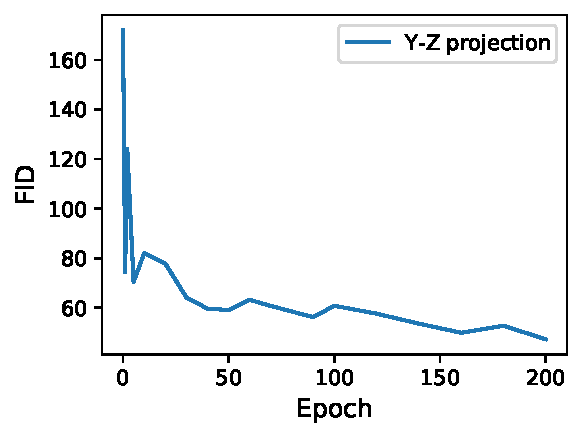
\includegraphics[width=\textwidth]{chapter4/fid_epoch-yz.pdf}
        %\caption{}
    \end{subfigure}
    \begin{subfigure}[t]{0.32\textwidth}
        \centering
        \hspace{-0.85cm}
        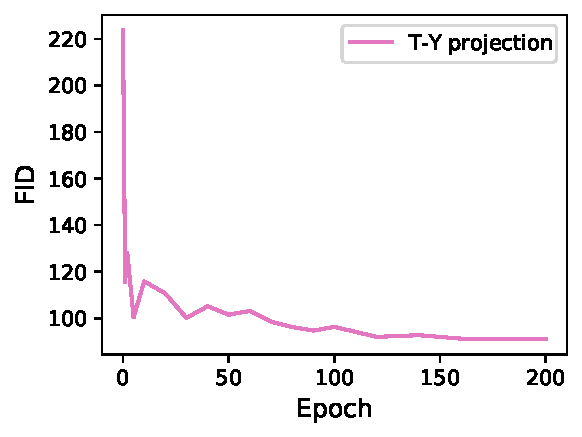
\includegraphics[width=\textwidth]{chapter4/fid_epoch-ty.pdf}
        %\caption{}
    \end{subfigure}
    \begin{subfigure}[t]{0.32\textwidth}
        \centering
        \hspace{-0.85cm}
        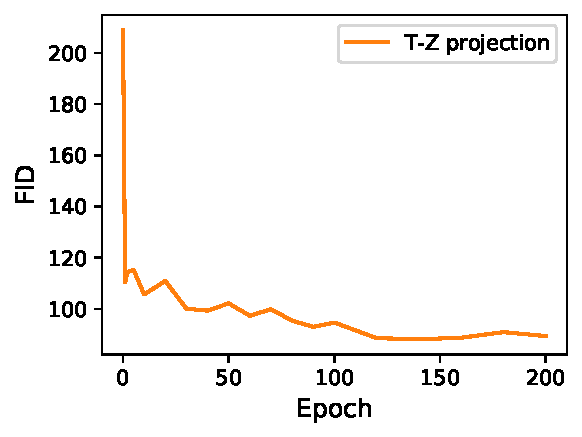
\includegraphics[width=\textwidth]{chapter4/fid_epoch-tz.pdf}
        %\caption{}
    \end{subfigure}
    \caption{
        Fréchet Inception Distance obtained from generated CDC hits over
        training epochs. Since the Inception network requires a 2D image as
        input, the hit data is projected along three axes and a separate FID
        is calculated for each projection.
    }
    \label{fig:FID_vs_epochs}
\end{figure}

The task of developing an independent quality metric for the CDC hit-generating
GAN was tackled by a pair of MSci students during a 6-month
project~\cite{noamandirene}.

As a baseline, the Inception~v3 model trained on the ImageNet dataset was used
to compute FID between generated and real samples. The network expects tensors
with two spatial dimensions and three channels as input. Hit positions are
discretised into a $300 \times 300$ grid and the three continuous features are
used as channels. 
The ordering of hits contains important information hence our distance metric
ought to use it. We can interpret the ordering as a third, temporal dimension.
However the Inception network cannot process 3D objects, hence we are forced to
project out one of the dimensions in order to compute FID.
Figure~\ref{fig:FID_vs_epochs} shows FID computed for each of the three
projections as a function of training iterations.


In order to process whole hit sequences rather than projections, two options
were considered: training a custom network which can take three-dimensional
tensors as input, and adding layers to the Inception network
and fine-tuning it.



\hl{150x150 is only for the 3D cnn, others use 300x300.}

A custom neural network is consequently developed to allow feature extraction
from entire unprojected hit sequences and provide a new distance metric specific
to the hit-generating GAN. In analogy with FID, the network is trained
independently from the GAN to classify hit samples. The categories are chosen to
be the same reconstructible and noise-like classes which we used to define what
data the GAN learns to generate. We expect such a classifier to rely on the
positioning and clustering of hit patterns to discriminate samples. Hence the
intermediate activations which will be used to compute the Fréchet distance
ought to be a representation of that information and hence help to define a
sensible distance metric.
Figure~\ref{fig:custom_distance_vs_epochs} shows \hl{...}.

\begin{figure}
    \centering
    \hl{FIG}
    %\includegraphics[width=0.6\textwidth]{}
    \caption{Custom distance metric applied to generated CDC hits over training epochs.}
    \label{fig:custom_distance_vs_epochs}
\end{figure}


\hl{t-SNE, examples of what GAN is modelling / not modelling?}

\hl{Transfer learning model?}




% The hit generation rate is X hits/s, whereas a traditional MC simulation
% starting from the POT collision creates X hits/s. If re-seeding is used to
% sample particles at the detector region boundary, X hits/s can be produced, so
% the efficiency gain is about 1e7. However the worry is not so much whether or
% not GANs can yield increase in efficiency (they can), but whether their output
% respects all the physical properties expected from MC data.

%\subsection{\hl{How GAN-generated hits are merged back into a dataset}}